\documentclass[letterpaper,11pt]{article}

\usepackage{latexsym}
\usepackage[empty]{fullpage}
\usepackage{titlesec}
\usepackage{marvosym}
\usepackage[usenames,dvipsnames]{color}
\usepackage{verbatim}
\usepackage{enumitem}
\usepackage[hidelinks]{hyperref}
\usepackage{fancyhdr}
\usepackage[english]{babel}
\usepackage{tabularx}
\usepackage{fontawesome5}
\usepackage{multicol}
\setlength{\multicolsep}{-3.0pt}
\setlength{\columnsep}{-1pt}
\input{glyphtounicode}

%new packages

\usepackage{fontenc}
\usepackage{amsmath}
\usepackage{amssymb}
\usepackage{graphicx}



%----------FONT OPTIONS----------

\pagestyle{fancy}
\fancyhf{} % clear all header and footer fields
\fancyfoot{}
\renewcommand{\headrulewidth}{0pt}
\renewcommand{\footrulewidth}{0pt}

% Adjust margins
\addtolength{\oddsidemargin}{-0.6in}
\addtolength{\evensidemargin}{-0.5in}
\addtolength{\textwidth}{1.19in}
\addtolength{\topmargin}{-.7in}
\addtolength{\textheight}{1.4in}

\urlstyle{same}

\raggedbottom
\raggedright
\setlength{\tabcolsep}{0in}

% Sections formatting
\titleformat{\section}{
  \vspace{-4pt}\scshape\raggedright\large\bfseries
}{}{0em}{}[\color{black}\titlerule \vspace{-5pt}]



% Ensure that generate pdf is machine readable/ATS parsable
\pdfgentounicode=1

%-------------------------
% Custom commands
\newcommand{\resumeItem}[1]{
  \item\small{
    {#1 \vspace{-2pt}}
  }
}

\newcommand{\classesList}[4]{
    \item\small{
        {#1 #2 #3 #4 \vspace{-2pt}}
  }
}

\newcommand{\resumeSubheading}[4]{
  \vspace{-2pt}\item
    \begin{tabular*}{1.0\textwidth}[t]{l@{\extracolsep{\fill}}r}
      \textbf{#1} & \textbf{\small #2} \\
      \textit{\small#3} & \textit{\small #4} \\
    \end{tabular*}\vspace{-7pt}
}

\newcommand{\resumeSubSubheading}[2]{
    \item
    \begin{tabular*}{0.97\textwidth}{l@{\extracolsep{\fill}}r}
      \textit{\small#1} & \textit{\small #2} \\
    \end{tabular*}\vspace{-7pt}
}

\newcommand{\resumeProjectHeading}[2]{
    \item
    \begin{tabular*}{1.001\textwidth}{l@{\extracolsep{\fill}}r}
      \small#1 & \textbf{\small #2}\\
    \end{tabular*}\vspace{-7pt}
}


\newcommand{\resumeSubItem}[1]{\resumeItem{#1}\vspace{-4pt}}

\renewcommand\labelitemi{$\vcenter{\hbox{\tiny$\bullet$}}$}
\renewcommand\labelitemii{$\vcenter{\hbox{\tiny$\bullet$}}$}

\newcommand{\resumeSubHeadingListStart}{\begin{itemize}[leftmargin=0.0in, label={}]}
\newcommand{\resumeSubHeadingListEnd}{\end{itemize}}
\newcommand{\resumeItemListStart}{\begin{itemize}}
\newcommand{\resumeItemListEnd}{\end{itemize}\vspace{-5pt}}




\begin{document}
\fontfamily{cmr}\selectfont
\begin{center}
\parbox{3.0cm}{%
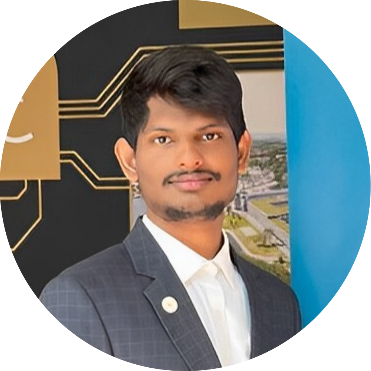
\includegraphics[width=2.7cm,clip]{images/resume_pic_m.png}}
}
\parbox{\dimexpr\linewidth-3.8cm\relax}{
\vspace{-20pt}
\begin{tabularx}{\linewidth}{L r} \\
    {\Huge \scshape  Venkata Sai Yakkshit Reddy Asodi}~
    \href{https://www.cedzlabs.com/yakkshit}{\vspace{1pt}}\\
      Berlin, Germany. \\ \vspace{1pt}
     \small \raisebox{-0.1\height}\faPhone\ +91 8179936156 ~ \href{mailto:saiyakkshit2001@gmail.com}{\raisebox{-0.2\height}\faEnvelope\  {saiyakkshit2001@gmail.com}} ~ 
    \href{https://linkedin.com/in/yakkshit/}{\raisebox{-0.2\height}\faLinkedin\ {yakkshit}}  ~
    \href{https://yakkshit.com/}{\raisebox{-0.2\height}\faGlobe\ {yakkshit.com}}  ~
    \href{https://github.com/yakkshit}{\raisebox{-0.2\height}\faGithub{ yakkshit}}
    \vspace{-8pt}
\end{tabularx}
}
\end{center}

\vspace{-23pt}

\section{Summary}
Tech-savvy Full Stack Developer with extensive experience in app development and artificial intelligence. Skilled in leading scalable tech projects and driving innovation, with a strong entrepreneurial mindset. Proven ability to build fast-paced startups and deliver results in high-pressure environments.

\section{Technical Skills}
\begin{itemize}[leftmargin=0.15in, label={}]
\item \textbf{Languages:} JavaScript (ES6+), Python, HTML5, CSS3
\item \textbf{Frameworks:} React, Next.js, Node.js, Django
\item \textbf{Tools:} Git, Docker, Kubernetes, Azure, AWS
\item \textbf{Deployment:} AWS, Azure, CI/CD pipelines
\end{itemize}

\section{Experience}
\resumeSubHeadingListStart
\resumeSubheading
{Circleup AG}{Dec 2023 -- Present}
{Lead Full Stack Engineer}{Zurich, Switzerland}
\vspace{-10pt}
\begin{itemize}
\item Led development of a nutrition coaching app, ensuring scalability and high performance for AI-driven services.
\item Collaborated closely with backend developers on API integrations and optimized the frontend for responsiveness and UX.
\item Enhanced the app's scalability and performance by optimizing cloud infrastructure.
\end{itemize}

\resumeSubheading
{Cedzlabs}{Mar 2023 -- Dec 2023}
{Full Stack Developer}{India}
\vspace{-10pt}
\begin{itemize}
\item Built and maintained full-stack web applications, focusing on seamless frontend experiences using Next.js and React.
\item Collaborated with cross-functional teams to deliver projects on time with agile methodologies.
\end{itemize}
\resumeSubHeadingListEnd

\section{Projects}
\resumeSubHeadingListStart
\resumeProjectHeading
{\textbf{AI Resume Tuner} $|$ \emph{Next.js, Azure, RAG}}{Aug 2023 -- Present}
\begin{itemize}
\item Developed an AI-powered resume generator utilizing Retrieval Augmented Generation (RAG) to create customized resumes based on candidate profiles and job descriptions.
\item Integrated cloud services using Azure to ensure seamless performance and scalability.
\end{itemize}

\resumeProjectHeading
{\textbf{Personal Portfolio Website} $|$ \emph{Next.js, AWS}}{Jan 2023}
\begin{itemize}
\item Built a fully responsive personal portfolio with enhanced UI/UX using Next.js and hosted on AWS.
\end{itemize}
\resumeSubHeadingListEnd

\section{Achievements}
\begin{itemize}
\item Successfully implemented agile methodologies across multiple projects, increasing team efficiency by 30\%.
\item Contributed to open-source projects in the areas of web development and design systems.
\item Regular participant in tech meetups, hackathons, and workshops on artificial intelligence.
\end{itemize}

\end{document}